\documentclass[times, utf8, diplomski]{fer}
\usepackage{booktabs}
\usepackage[croatian]{babel}
\usepackage[utf8]{inputenc}
\usepackage{pdfpages}

\setcounter{secnumdepth}{3}
\setcitestyle{numbers}
\graphicspath{ {./images/} }

\begin{document}

\thesisnumber{1373}

\title{Analiza i usporedba sigurnosnih mehanizama u Internetu stvari}

\author{Filip Ptiček}

\maketitle

% Ispis stranice s napomenom o umetanju izvornika rada. Uklonite naredbu \izvornik ako želite izbaciti tu stranicu.
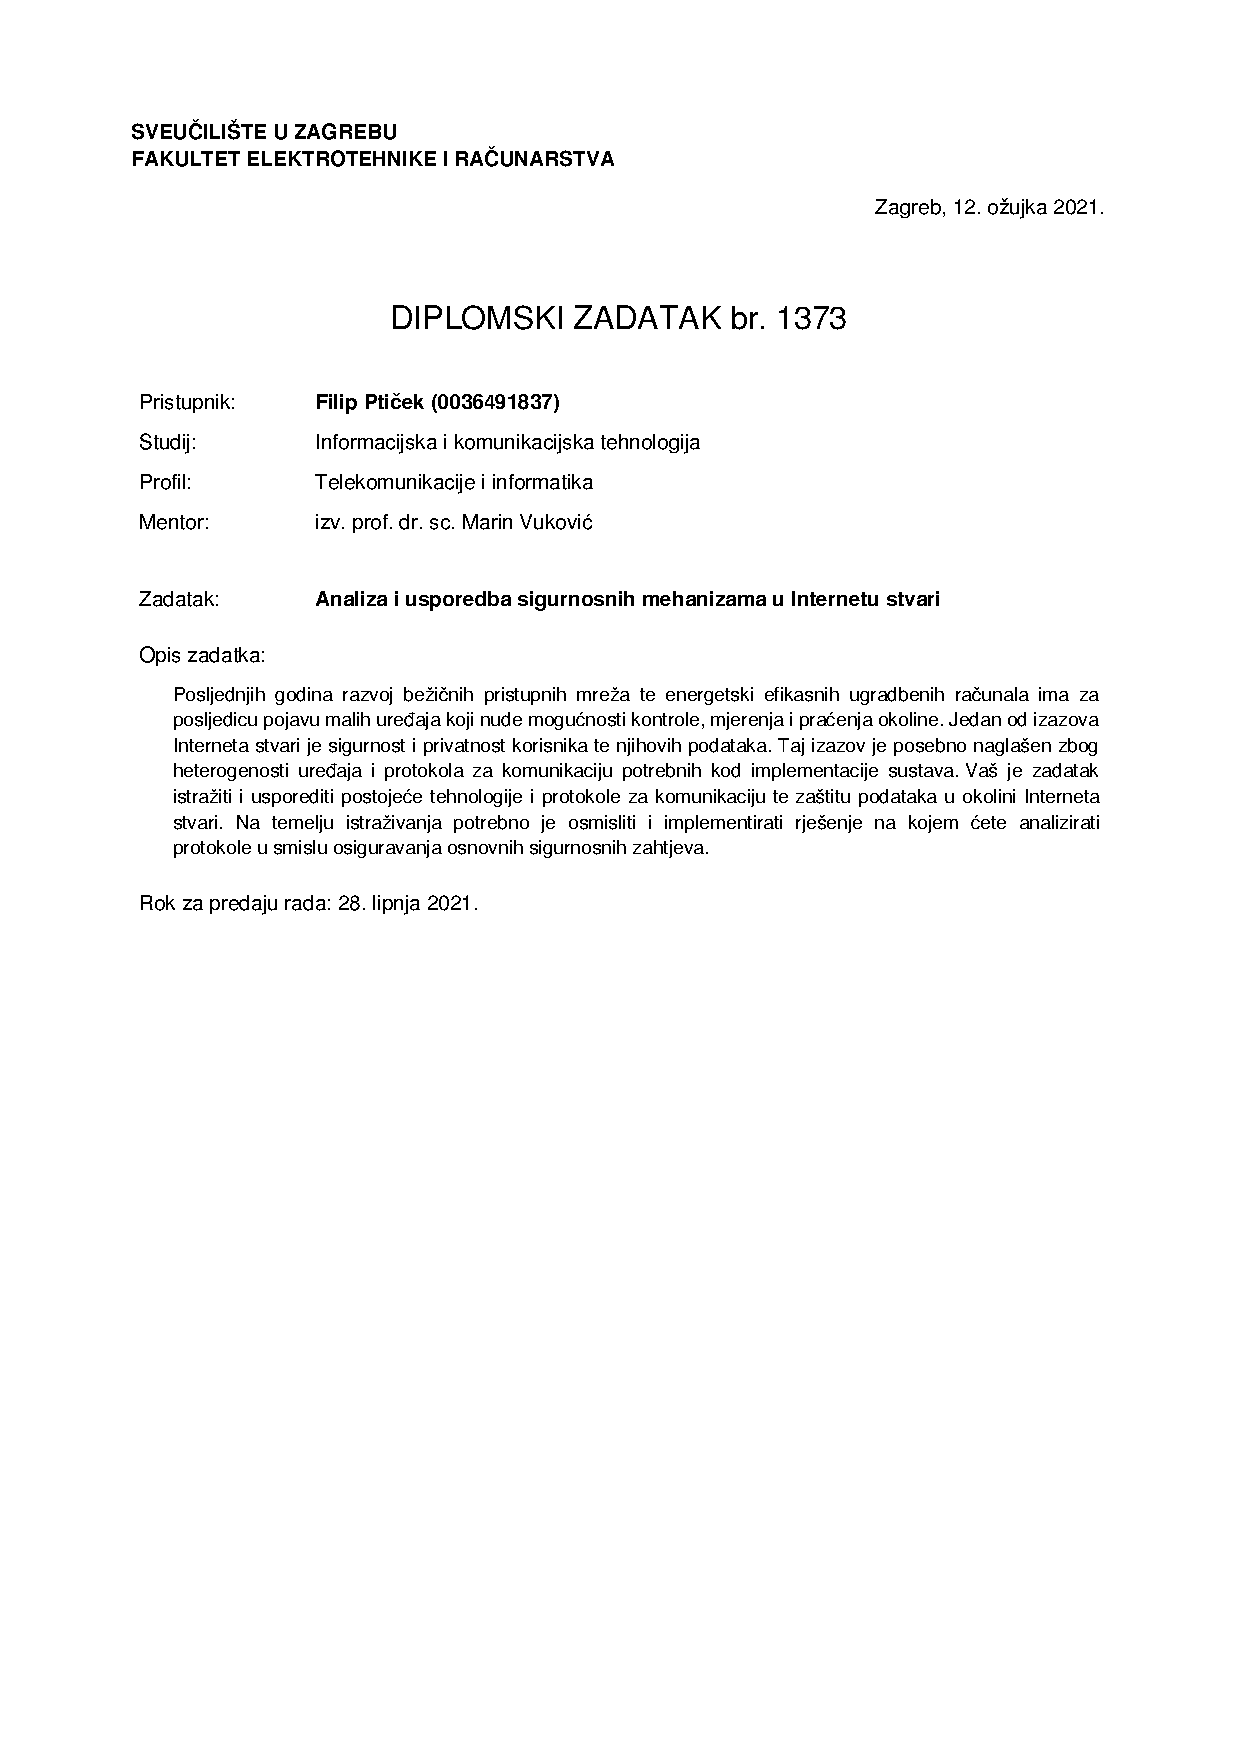
\includepdf[pages=-,fitpaper=true]{zadatak.pdf}

% Dodavanje zahvale ili prazne stranice. Ako ne želite dodati zahvalu, naredbu ostavite radi prazne stranice.
\zahvala{}

\tableofcontents

\chapter{Uvod}
Uvod u rad

\chapter{Internet stvari}

\section{Definicija}

\section{Model IoT sustava}

\section{Čimbenici u sustavu}

\section{Programske platforme}


\section{Otvorena pitanja}

\subsection{Sigurnost}

\subsection{Privatnost}

\subsection{Skalabilnost}

\subsection{Decentraliziranost}

\section{Primjene}

\subsection{Područja primjene}

\subsection{Zahtijevi sustava s obzirom na primjenu}

\section{Trendovi}


\chapter{Sigurnosni zahtijevi u Internet stvarima}

\section{OWASP Top 10}
The Open Web Application Security Project® (OWASP) je neprofitna organizacija čiji je cilj napredak i poboljšanje računalne sigurnosti informacijskih sustava. OWASP kroz svoje projekte otvorenog koda vođenih putem razvojne zajednice radi na poboljšanju sigurnosti Interneta.

\emph{OWASP Internet of Things Project} je projekt osmišljen kako bi pomogao proizvođačima, programerima i potrošačima bolji uvid i razumijevanje u sigurnosne probleme vezane uz Internet stvari. Na taj način korisnici u bilo kojem dijelu razvojnog procesa mogu donositi bolje odluke kod razvoja, deployanja i pristupanja tehnologijama Interneta stvari.\citep{owasp1} 2018. godine izlazi OWASP IoT Top 10 lista koja reprezentira deset najčešćih ranjivosti Internet stvari sustava. Svih deset sigurnosnih ranjivosti su navedeni u nastavku uz opis sigurnosnih zahtijeva koji bi trebali spriječiti te ranjivosti i sigurnosne propuste. 


\subsection{Slabe, pogodljive ili tvrdo kodirane lozinke}
Najčešći uzrok

\subsection{Nesigurni mrežni servisi}

\subsection{Nesigurna sučelja ekosustava}

\subsection{Nedostatak mehanizama za sigurnosna ažuriranja}

\subsection{Upotreba nesigurnih ili zastarijelih komponenti}

\subsection{Nedovoljna zaštita privatnosti}

\subsection{Nesigurni prijenos i pohrana podataka}

\subsection{Nedostatak mogućnosti upravljanja uređajima}

\subsection{Nesigurne zadane postavke}

\subsection{Nedostatak fizičke sigurnosti}

\section{Primjeri sigurnosnih napada i propusta}

\chapter{Analiza i usporedba protokola}

\section{IoT stack}
Iot stack

\section{Senzori i uređaji}
Senzori

\subsection{Analiza uređaja}
Uređaji

\subsubsection{Senzori s komunikacijskim modulom}

\subsubsection{Pristupni uređaji}

\subsection{Usporedba sigurnosnih mehanizama i primjena}

\section{Sloj podatkovne poveznice}

\subsection{Analiza protokola}

\subsubsection{WiFi}

\subsubsection{BLE}

\subsubsection{RFID\textbackslash NFC}

\subsubsection{ZigBee}

\subsubsection{LTE}

\subsubsection{SigFox}

\subsubsection{LoRaWan}

\subsection{Usporedba sigurnosnih mehanizama i primjena}

\section{Mrežni sloj}

\subsection{Analiza protokola}
Neki protokoli

\subsubsection{IPv4}

\subsubsection{IPv6}

\subsection{Usporedba sigurnosnih mehanizama i primjena}

\section{Transportni sloj}

\subsection{Usporedba primjena protokola}

\section{Aplikacijski sloj}

\subsection{Analiza protokola}

\subsubsection{HTTP/S}

\subsubsection{COAP}

\subsubsection{MQTT}

\subsection{Usporedba sigurnosnih mehanizama i primjena}

\chapter{Sustav za praćenje tjelesne temperature}

\section{Arhitektura sustava}

\section{Korišteni razvojni alati i uređaji}

\section{Opis rada sustava}

\section{Sigurnostna analiza sustava}


\chapter{Zaključak}
Zaključak.

\bibliographystyle{fer}
\bibliography{literatura}

\begin{sazetak}
Sažetak na hrvatskom jeziku.

\kljucnerijeci{Ključne riječi, odvojene zarezima.}
\end{sazetak}

% TODO: Navedite naslov na engleskom jeziku.
\engtitle{Title}
\begin{abstract}
Abstract.

\keywords{Keywords.}
\end{abstract}

\end{document}